\documentclass[conference]{IEEEtran}
\usepackage{amsmath,amssymb,graphicx,booktabs}
\usepackage[hidelinks]{hyperref}
% Generated from results/metrics.json; do not edit.
\newcommand{\TestAcc}{99.9902}
\newcommand{\TestIoU}{0.998556}
\newcommand{\TrainAcc}{99.9901}
\newcommand{\TrainIoU}{0.998548}
\newcommand{\TrainBCE}{0.000306}
\newcommand{\TestBCE}{0.000303}
\newcommand{\MeanIoU}{0.998146}
\newcommand{\TrainSeconds}{37.3}
\newcommand{\Parameters}{116,753}
\newcommand{\BackgroundAcc}{93.2028}
\newcommand{\TP}{222,635}
\newcommand{\TN}{3,053,843}
\newcommand{\FP}{226}
\newcommand{\FN}{96}
\newcommand{\CircleAcc}{99.9983}
\newcommand{\CircleIoU}{0.999735}
\newcommand{\SquareAcc}{99.9866}
\newcommand{\SquareIoU}{0.998490}
\newcommand{\TriangleAcc}{99.9856}
\newcommand{\TriangleIoU}{0.997113}

\newcommand{\StudentLine}{}
\InputIfFileExists{author_local.tex}{}{}
\title{Binary Segmentation of Synthetic Shapes\protect\\with a Small U-Net}
\author{\IEEEauthorblockN{Keru Chen}
\IEEEauthorblockA{Arizona State University\\Assignment 3: U-Net Segmentation\StudentLine}}
\begin{document}
\maketitle
\begin{abstract}
We train a two-level U-Net to segment circles, squares, and triangles in $128\times128$ grayscale images. With 1,000 training images, 200 independent test images, and 15 epochs of binary cross-entropy training, the final model achieves \TestAcc\% test accuracy and \TestIoU\ foreground intersection over union (IoU). Similar training and test performance suggests no obvious fitting problem under this generator. The disjoint intensity ranges make this a controlled exercise; the results do not establish performance on natural images.
\end{abstract}



\section{Task and Data Generation}
Binary segmentation requires a spatially aligned decision at every pixel. A reduced U-Net~\cite{unet} combines spatial context with features retained at the original resolution. The target is foreground membership; shape labels only balance the dataset and summarize results.

Each image contains one fully visible shape on a dark background. A seeded NumPy generator samples integer background intensities uniformly from $[0,55]$ and object intensities from $[200,255]$, independently at each pixel. Pillow rasterizes the geometry into a strict $\{0,1\}$ mask without antialiasing. Input intensities are divided by 255 before training.

Circle radii are sampled from the integers 10--25 pixels, and square half-sides from 12--25 pixels. For triangles, three approximately evenly spaced angles and perturbed radii generate nondegenerate vertices; the maximum pairwise vertex distance is scaled to a uniform 30--60 pixels before rasterization. Squares and triangles are rotated by a uniform angle in $[0,2\pi)$ and translated to a random position that preserves a border margin. Circle rotation has no visual effect. Pixel rounding introduces at most small deviations from continuous polygon dimensions.

Training and test sets use independent seeds 2026 and 2027. Their circle/square/triangle counts are 334/333/333 and 67/67/66, respectively. The 1,000 training images remain fixed across epochs; only their order is shuffled. No external dataset, pretrained weights, or additional augmentation is used.

\section{Network and Training}
\begin{figure}[t]
\centering
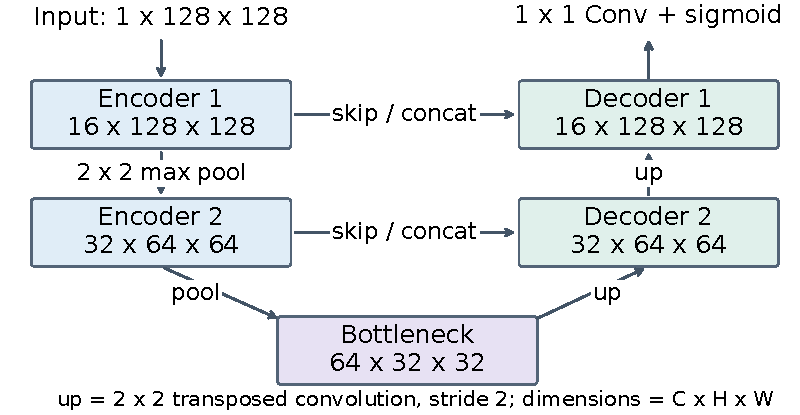
\includegraphics[width=\columnwidth]{../figures/architecture.pdf}
\caption{Two-level U-Net with \Parameters\ trainable parameters. Concatenation joins each upsampled feature map with the encoder map at the same resolution.}
\label{fig:unet}
\end{figure}
\begin{figure*}[t]
\centering
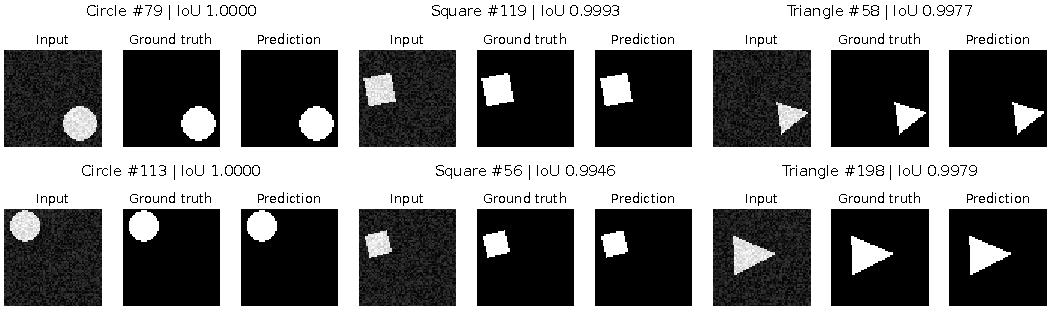
\includegraphics[width=0.94\textwidth]{../figures/test_examples.pdf}
\caption{Six test examples selected uniformly without replacement within each shape using seed 2028, independently of prediction quality. Each triplet shows the grayscale input, ground truth, and prediction. The three groups show circles, squares, and triangles, with two examples per shape. Test indices are zero-based.}
\label{fig:examples}
\end{figure*}
The encoder has 16 and 32 channels, followed by a 64-channel bottleneck (Fig.~\ref{fig:unet}). Each feature block applies two $3\times3$ convolutions with padding one and a ReLU after each convolution. Two $2\times2$ max-pooling operations reduce the spatial resolution to $32\times32$. Each decoder stage uses a $2\times2$, stride-two transposed convolution, concatenates the corresponding encoder features, and applies a double-convolution block. The decoder returns to 32 and then 16 channels. Skip connections preserve spatial detail that pooling can discard. A final $1\times1$ convolution produces one logit per pixel; a sigmoid converts logits to foreground probabilities.

For target $y_i\in\{0,1\}$ and probability $p_i$, training minimizes the average binary cross-entropy over all $M$ pixels in a mini-batch:
\begin{equation}
\mathcal{L}=-\frac{1}{M}\sum_{i=1}^{M}\left[y_i\log p_i+(1-y_i)\log(1-p_i)\right].
\end{equation}
The implementation uses \texttt{BCEWithLogitsLoss}, which combines the sigmoid and cross-entropy stably. Adam uses learning rate $10^{-3}$, $\beta_1=0.9$, $\beta_2=0.999$, $\epsilon=10^{-8}$, and zero weight decay. Batch size is 32; the final batch contains eight images. Initialization and shuffling use seed 42. There is no scheduler, dropout, batch normalization, or class weighting.

\begin{figure}[t]
\centering
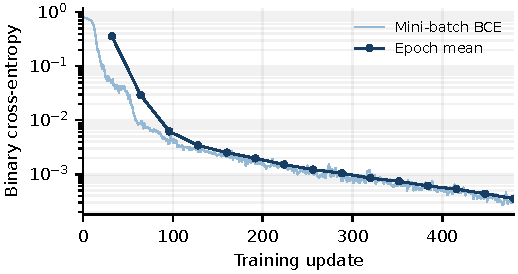
\includegraphics[width=\columnwidth]{../figures/learning_curve.pdf}
\caption{Training loss versus optimizer updates on a logarithmic vertical scale. Epoch means weight each batch by its number of images. The curve contains all 480 updates.}
\label{fig:loss}
\end{figure}
Training stops after the preselected 15 epochs, yielding 480 optimizer updates. The final checkpoint is evaluated without selecting a checkpoint or threshold on the test set. This follows the assignment's allowance to omit a validation split. Training took \TrainSeconds\ seconds on an Apple M4 using PyTorch 2.9.0 with the MPS backend, excluding data generation and final evaluation. Figure~\ref{fig:loss} shows the full optimization trajectory; the epoch-average loss decreases from 0.357722 to 0.000351.



\section{Evaluation and Results}
Probabilities at least 0.5 are classified as foreground. We pool pixel counts over the 200 test images before calculating metrics. A true positive (TP) is correctly predicted foreground, a true negative (TN) is correctly predicted background, a false positive (FP) is background predicted as foreground, and a false negative (FN) is missed foreground. With $N=200\times128\times128=3{,}276{,}800$ pixels,
\begin{equation}
\mathrm{Accuracy}=\frac{TP+TN}{N},\qquad
\mathrm{IoU}=\frac{TP}{TP+FP+FN}.
\end{equation}
IoU evaluates foreground overlap and is therefore informative when most pixels are background. An all-background prediction reaches \BackgroundAcc\% accuracy but zero IoU on this test set.

\begin{table}[t]
\centering
\caption{Final-checkpoint metrics. Shape-specific rows pool the pixels of that shape. Accuracy is a percentage; IoU is a fraction.}
\label{tab:results}
\begin{tabular}{lrrr}
\toprule
Split / shape & Images & Accuracy (\%) & Foreground IoU\\
\midrule
Training, all & 1,000 & \TrainAcc & \TrainIoU\\
Test, all & 200 & \TestAcc & \TestIoU\\
\midrule
Test, circles & 67 & \CircleAcc & \CircleIoU\\
Test, squares & 67 & \SquareAcc & \SquareIoU\\
Test, triangles & 66 & \TriangleAcc & \TriangleIoU\\
\bottomrule
\end{tabular}
\end{table}

The test confusion counts are $TP=\TP$, $TN=\TN$, $FP=\FP$, and $FN=\FN$, for 322 misclassified pixels in total. They produce \TestAcc\% accuracy and \TestIoU\ IoU (Table~\ref{tab:results}). The unweighted mean of the 200 individual image IoUs is \MeanIoU; it differs from pooled IoU because small and large objects receive equal weight. Circles have the highest pooled IoU, while triangles have the lowest in this run. Figure~\ref{fig:examples} shows the requested two examples per shape without selecting for visual quality.

At the final checkpoint, training and test BCE are \TrainBCE\ and \TestBCE, respectively. Training IoU (\TrainIoU) is close to test IoU (\TestIoU). Low training loss, high foreground overlap, and this small gap provide no obvious evidence of underfitting or overfitting on the generated distribution. They do not replace evaluation across seeds or on a different image distribution.

\section{Discussion and Reproducibility}
The generator deliberately separates object and background intensities. A fixed intensity threshold $I\geq128$ therefore recovers every test mask exactly, attaining 100\% accuracy and IoU 1. This reference exposes the task's simplicity: the U-Net learns the requested mapping, but is unnecessary for optimal performance on this particular generator. More realistic evaluation would require overlapping intensity distributions, textured backgrounds, occlusion, or multiple objects. Such settings are outside the reported experiment.

The implementation, checkpoint, per-update losses, per-image counts, random seeds, dataset hashes, and figure-generation scripts are available at the following public repository:
\begin{center}
\small\url{https://github.com/CLIVERCHEN/assignment3-unet-segmentation}
\end{center}
The README gives reproduction commands, including checkpoint evaluation without retraining. Results describe one fixed run; training numerics can vary across hardware and backend versions.

\begin{thebibliography}{1}
\bibitem{unet} O. Ronneberger, P. Fischer, and T. Brox, ``U-Net: Convolutional networks for biomedical image segmentation,'' in \emph{MICCAI}, 2015, pp. 234--241. [Online]. Available: \url{https://arxiv.org/abs/1505.04597}
\end{thebibliography}
\end{document}
